\documentclass{easychair}

\newcommand{\todo}[1]{$\langle\langle$#1 $\rangle\rangle$}
\usepackage{hyperref}
\usepackage{xspace}

\newcommand{\qflra}{QF\_LRA}
\newcommand{\qflia}{QF\_LIA}
\newcommand{\qfuf}{QF\_UF}
\newcommand{\qfbv}{QF\_BV}
\newcommand{\qfrdl}{QF\_RDL}
\newcommand{\qfidl}{QF\_IDL}
\newcommand{\qfuflra}{QF\_UFLRA}
\newcommand{\qfuflia}{QF\_UFLIA}
\newcommand{\qfax}{QF\_AX}
\newcommand{\qfauflia}{QF\_AUFLIA}
\newcommand{\qfauflra}{QF\_AUFLRA}
\newcommand{\qfalia}{QF\_ALIA}
\newcommand{\qfalra}{QF\_ALRA}

\newcommand{\opensmt}{\textsc{OpenSMT}\xspace}

\title{The OpenSMT Solver in SMT-COMP 2023}
\author{
Martin Blicha\inst{1,3} \and
Konstantin I. Britikov\inst{1} \and
Antti E. J. Hyv{\"a}rinen\inst{2} \and
Rodrigo Otoni\inst{1} \and 
Natasha Sharygina\inst{1} \\
}
\institute{Universit{\`a} della Svizzera italiana (USI), Lugano,
Switzerland \and Certora, Isreal \and Charles University, Prague, Czech Republic}
\date{}
\titlerunning{The OpenSMT Solver}
\authorrunning{Blicha et al.}
\begin{document}
\maketitle

\section{Overview}

\opensmt~\cite{HyvarinenMAS16} is a T-DPLL based SMT
solver~\cite{NieuwenhuisOT:JACM06} that has been developed at USI,
Switzerland, since 2008.  The solver is written in {\tt C++} and
currently supports the quantifier-free logics of equality with
uninterpreted functions (\qfuf), linear real and integer arithmetic
(\qflra, \qflia), arrays (\qfax) and their combinations (\qfuflra, \qfuflia, \qfalia, \qfalra, \qfauflia, \qfauflra).
It has a specialized solver for real and integer difference logics (\qfrdl,
\qfidl). \opensmt also supports some aspects of bit-vector logic (\qfbv).

In comparison to 2022, the 2023 competition entry supports a combination of arrays with linear arithmetic and uninterpreted functions(\qfalia, \qfalra, \qfauflia, \qfauflra). 
Additionally, the lookahead engine of \opensmt now supports interpolation and incremental solving.
Performance of a lookahead engine has been improved with a new heuristic.

\opensmt features not exercised in the competition include support for a
wide range of interpolation algorithms for propositional
logic~\cite{AltFHS:VSTTE2015}, linear real
arithmetic~\cite{BlichaHKS19}, and uninterpreted
functions~\cite{AltHAS:FMCAD17} (available also in the incremental
mode); an experimental look\-ahead-based search
algorithm~\cite{HyvarinenMSCS18} as an alternative to the more standard
CDCL algorithm; and features that support search-space partitioning in
particular designed for parallel solving~\cite{HyvarinenMS:SAT15}.
\opensmt is now also able to efficiently produce proofs of
unsatisfiability~\cite{OtoniBEHS:DAC21}, although this feature is not merged to the main repository.

\iffalse % No parallel submission this year
\section{Cloud and Parallel Solver}
The parallel version of \opensmt, called SMTS, runs on our parallelization infrastructure described in~\cite{MarescottiHS18}. The system is a client-server architecture that communicates with a custom protocol over TCP/IP. Parallel solving features include the complete implementation of the partition tree protocol with clause sharing. On a high level, the parallel solver partitions the instance dynamically on-demand and allows clauses to be shared between solvers working on different instances whenever this is allowed based on the information in the solvers. The dynamic partitioning is implemented as an iteration in a tree of consisting of partitioned instances, and the instances in inner nodes are considered equally to those in the leaves. This aproach guarantees under reasonable assumptions on the instance’s run time distribution that the parallel solver will not be slower than the sequential solver ~\cite{HyvarinenMS:SAT15}. For a fair and load-balanced scheduling of solving of the partitions, the solvers are distributed over the instances on parameters such as whether the instance has already been attempted, how many solvers are working on the instance, and how deep in the tree the instance is.
\begin{figure}
    \centering
    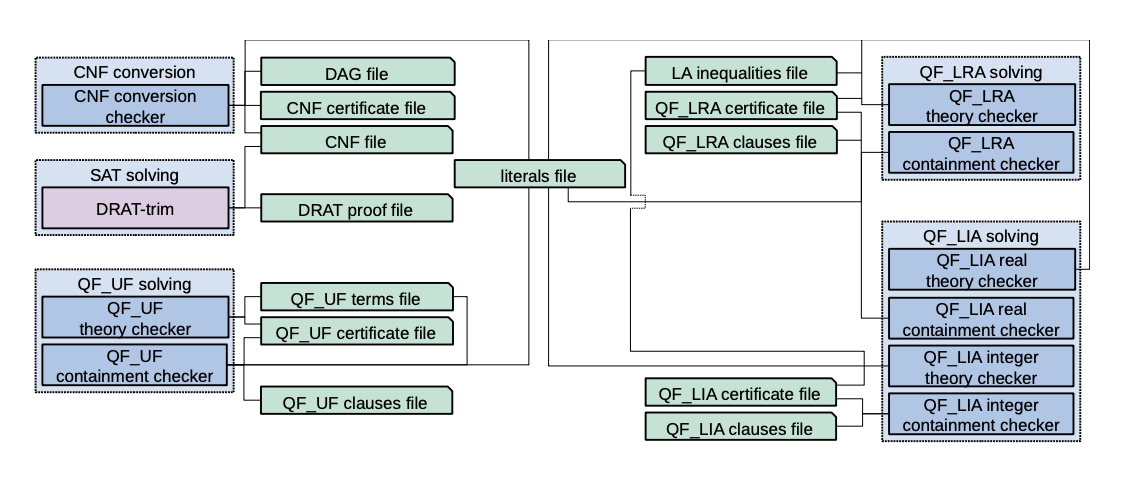
\includegraphics[angle=0, width=12cm]{Architecture.png}
    % \caption{Caption}
    \label{fig:architecture}
\end{figure}
We support running the solver in the in AWS infrastructure, but it can also be run, e.g., in multi-core environments. We have entered two versions of the solver to the cloud and parallel tracks: SMTS portfolio which randomises the SAT solver by choosing 2\% of the decision variables randomly; and SMTS cube-and-conquer, which uses the parallelization tree~\cite{HyvarinenMS:SAT15} approach to implement a version of search-space-partitioning.


The cloud version of \opensmt, called SMTS, is designed to run in AWS
infrastructure and runs on our parallelization infrastructure described
in~\cite{MarescottiHS18}.
%
We have entered two versions of the solver to the experimental cloud
track: {\em SMTS portfolio} which randomises the SAT solver by choosing
2\% of the decision variables randomly; and {\em SMTS cube-and-conquer},
which uses the {\em parallelization tree}~\cite{HyvarinenMS:SAT15}
approach to implement a version of search-space-partitioning.
\fi

\section{External Code and Contributors}

The SAT solver driving \opensmt is based on the MiniSAT
solver~\cite{EenS:SAT03}, and the rational number implementation is
inspired by a library written by David Monniaux.  Several people have
directly contributed to the \opensmt code.  In alphabetical order, the
major contributors are
%
Leonardo Alt (Ethereum Foundation),
Sepideh Asadi (USI),
Masoud Asadzade (USI),
Martin Blicha (USI, Charles University),
Konstantin I.~Britikov (USI),
Roberto Bruttomesso (Cybersecurity / Nozomi Networks),
Antti E.~J.~Hyv{\"a}rinen (Certora),
Andrew Jones (Vector),
V{\'a}clav Lu{\v n}{\'a}k (Charles University),
Matteo Marescotti (Meta),
Rodrigo Benedito Otoni (USI),
Edgar Pek (University of Illinois, Urbana-Champaign),
Simone Fulvio Rollini (United Technologies Research Center),
Parvin Sadigova (King's College London),
Mate Soos (Ethereum Foundation),
Michal Tarina
and Aliaksei Tsitovich (Sonova).
%
The solver is being developed in Natasha Sharygina's software
verification group at USI.

\section{Utilization}

\opensmt is used in a range of projects as a back-end solver.
Most notably, it is a basis for a new CHC solver Golem which scored among the top solvers
in LIA-Lin, LIA-Nonlin, and LRA-TS tracks in the last three editions of CHC-COMP~\cite{}
\opensmt also forms the basis of the model checkers HiFrog~\cite{AltACMFHS17} and
UpProver~\cite{Asadi_2020b}.
It was also used as an interpolation engine of the Sally model
checker~\cite{JovanovicD:FMCAD16}.

\section{Availability}
The source code repository and more information on the solver is
available at

\begin{itemize}
    \item \url{https://github.com/usi-verification-and-security/opensmt}
        and
    \item \url{https://verify.inf.usi.ch/opensmt}
\end{itemize}

\iffalse
in chronological order, work on interpolation 
algorithms~\cite{BlichaHKS19,AltHAS17,JancikAFHKS16,AsadiBFHESC18}
and parallel SMT 
solving~\cite{HyvarinenMSCS18,MarescottiHS18,HyvarinenMS:SAT15}.
OpenSMT2 is
used as the back-end in model-checking tools
HiFrog~\cite{AltACMFHS17},
eVolCheck~\cite{FSS_TACAS13}, 
FunFrog~\cite{SFS_ATVA12}, and
PeRIPLO~\cite{RolliniAFHS:LPAR2013,AltFHS:VSTTE2015}.
OpenSMT2 is a supported engine in the parallel 
solving framework SMTS~\cite{MarescottiHS16}.

\section{Acknowledgements}
We thank everyone who helped
developing OpenSMT2. In particular,
Leonardo Alt,
Sepideh Asadi,
Martin Blicha,
Roberto Bruttomesso,
Antti E. J. Hyv{\"a}rinen,
Matteo Marescotti,
Edgar Pek,
Simone Fulvio Rollini, 
Parvin Sadigova,
Natasha Sharygina,
Aliaksei Tsitovich.
\fi

\bibliography{abstract}
\bibliographystyle{plain}

\end{document}
